\documentclass[tikz,border=5pt]{standalone}
\usepackage{pgfplots}
\usetikzlibrary{arrows.meta}
\pgfplotsset{compat=1.18}

\definecolor{corba}{HTML}{365FB3}

\begin{document}
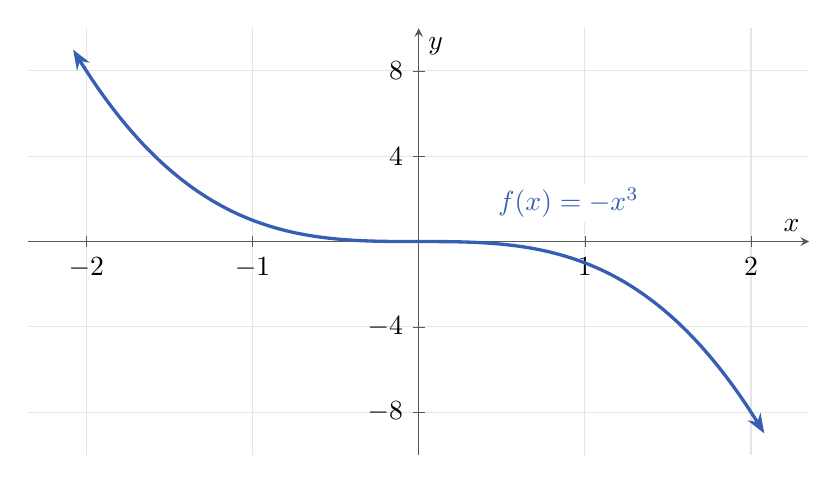
\begin{tikzpicture}
  \begin{axis}[
    width=11.5cm,
    height=7cm,
    axis lines=middle,
    xmin=-2.35,
    xmax=2.35,
    ymin=-10,
    ymax=10,
    xlabel={$x$},
    ylabel={$y$},
    xtick={-2,-1,1,2},
    ytick={-8,-4,4,8},
    axis line style={black!65},
    tick style={black!65},
    grid=major,
    grid style={black!10},
    clip=false,
  ]
    \addplot[
      corba,
      very thick,
      {Stealth[length=2.5mm]}-{Stealth[length=2.5mm]},
      domain=-2.08:2.08,
      samples=180
    ] {-x^3};

    \node[corba, fill=white, inner sep=1.5pt, anchor=west]
      at (axis cs:0.45,1.8) {$f(x)=-x^3$};
  \end{axis}
\end{tikzpicture}
\end{document}
